% validation_EN.tex — WAC (Windows Artefacts Collector) validation report, English edition.
% The French edition is validation_FR.tex, in this folder: both are maintained together,
% section for section.
%
% Build (XeLaTeX, two passes for the cover page and the table of contents):
%     latexmk -xelatex validation_EN.tex
% The cover page is ../cover_validation_EN.png, derived from ../cover_EN.png by
% ../retitle-cover.py. The layout is ../wac-style.tex, shared with every WAC document.
%
% This report says WHAT is verified and what it guarantees; how to run each test
% by hand is in the testing guide (../tests/testing_EN.tex).

\documentclass[11pt,a4paper,oneside]{report}

% ---------------------------------------------------------------- language and labels
\usepackage[english]{babel}
\newcommand{\wacdoctitle}{Validation report}
\newcommand{\wacpageof}{of}
\newcommand{\wacnotetitle}{Keep in mind}
\newcommand{\wacwarningtitle}{Limit}
% Layout shared with every WAC document.
% wac-style.tex — layout shared by every WAC document (user manuals, testing
% guides), French and English editions alike: one copy, so that they cannot
% drift apart.
%
% A document sets, BEFORE % wac-style.tex — layout shared by every WAC document (user manuals, testing
% guides), French and English editions alike: one copy, so that they cannot
% drift apart.
%
% A document sets, BEFORE % wac-style.tex — layout shared by every WAC document (user manuals, testing
% guides), French and English editions alike: one copy, so that they cannot
% drift apart.
%
% A document sets, BEFORE \input{../wac-style.tex}:
%   \usepackage[<language>]{babel}
%   \newcommand{\wacdoctitle}{...}      running header: "WAC — <title>"
%   \newcommand{\wacpageof}{...}        footer: "Page N <of> M"
%   \newcommand{\wacnotetitle}{...}     default title of the "note" box
%   \newcommand{\wacwarningtitle}{...}  default title of the "attention" box
% and AFTER it its \hypersetup (PDF title, author, subject).

% ---------------------------------------------------------------- fonts, language
\usepackage{fontspec}
\setmainfont{Noto Sans}
\setmonofont{DejaVu Sans Mono}[Scale=0.84]

% ---------------------------------------------------------------- layout
\usepackage[top=26mm,bottom=26mm,left=24mm,right=22mm,headheight=14pt]{geometry}
\usepackage{graphicx}
\graphicspath{{../}}
\usepackage{xcolor}
\usepackage{tikz}
\usepackage{booktabs,tabularx,longtable,array}
\usepackage{enumitem}
\usepackage{fancyhdr}
\usepackage{titlesec}
\usepackage[most]{tcolorbox}
\usepackage{listings}
\usepackage{url}
\usepackage{lastpage}
\usepackage[hidelinks,unicode,pdfpagelabels]{hyperref}

% Colours sampled from the cover page
\definecolor{marine}{HTML}{0A1A33}
\definecolor{bleu}{HTML}{2F6DB5}
\definecolor{accent}{HTML}{1F66D1}
\definecolor{fond}{HTML}{EEF3FA}
\definecolor{alerte}{HTML}{B3261E}
\definecolor{fondalerte}{HTML}{FBEDEC}
\definecolor{gris}{HTML}{5B6573}

\setlength{\parindent}{0pt}
\setlength{\parskip}{0.55em}
\linespread{1.08}
\setlist{itemsep=0.25em,topsep=0.35em}
\urlstyle{tt}
\renewcommand{\arraystretch}{1.25}
% Left-aligned table columns: justified narrow columns opened wide gaps
% between words.
\newcolumntype{L}[1]{>{\raggedright\arraybackslash}p{#1}}
% Monospaced file and field names cannot be hyphenated: let the line's spaces
% stretch instead.
\setlength{\emergencystretch}{3em}

% Headings
\titleformat{\chapter}[display]
  {\color{marine}\bfseries\raggedright}
  {\color{bleu}\large\MakeUppercase{\chaptertitlename}~\thechapter}
  {0.3em}
  {\Huge}[{\color{accent}\titlerule[2pt]}]
\titlespacing*{\chapter}{0pt}{0pt}{1.6em}
\titleformat{\section}{\color{marine}\Large\bfseries}{\color{bleu}\thesection}{0.8em}{}
\titleformat{\subsection}{\color{marine}\large\bfseries}{\color{bleu}\thesubsection}{0.7em}{}
\titleformat{\subsubsection}{\color{bleu}\normalsize\bfseries}{}{0em}{}

% Headers and footers
\pagestyle{fancy}
\fancyhf{}
\fancyhead[L]{\small\color{gris}WAC — \wacdoctitle}
\fancyhead[R]{\small\color{gris}\leftmark}
% Footer: "Page N of M" (the word set by \wacpageof), readable. A bare, small, light-grey number went
% unnoticed.
\newcommand{\piedpage}{\small\color{marine}\textbf{Page \thepage}\ \wacpageof\ \pageref*{LastPage}}
\fancyfoot[C]{\piedpage}
\renewcommand{\footrulewidth}{0.4pt}
\renewcommand{\footrule}{\hbox to\headwidth{\color{fond}\leaders\hrule height \footrulewidth\hfill}}
\renewcommand{\headrulewidth}{0.4pt}
\renewcommand{\headrule}{\hbox to\headwidth{\color{fond}\leaders\hrule height \headrulewidth\hfill}}
\renewcommand{\chaptermark}[1]{\markboth{#1}{}}
\fancypagestyle{plain}{\fancyhf{}\fancyfoot[C]{\piedpage}\renewcommand{\headrulewidth}{0pt}}

% Boxes
\newtcolorbox{note}[1][\wacnotetitle]{enhanced,breakable,colback=fond,colframe=bleu,
  boxrule=0pt,leftrule=3pt,arc=0pt,left=8pt,right=8pt,top=6pt,bottom=6pt,
  title={\bfseries #1},coltitle=bleu,colbacktitle=fond,attach title to upper={\par\smallskip}}
\newtcolorbox{attention}[1][\wacwarningtitle]{enhanced,breakable,colback=fondalerte,colframe=alerte,
  boxrule=0pt,leftrule=3pt,arc=0pt,left=8pt,right=8pt,top=6pt,bottom=6pt,
  title={\bfseries #1},coltitle=alerte,colbacktitle=fondalerte,attach title to upper={\par\smallskip}}

% Code
\lstset{basicstyle=\ttfamily\small,columns=fullflexible,keepspaces=true,
  backgroundcolor=\color{fond},frame=l,framerule=3pt,rulecolor=\color{bleu},
  xleftmargin=9pt,framexleftmargin=6pt,aboveskip=0.8em,belowskip=0.8em,
  breaklines=true,breakatwhitespace=false,showstringspaces=false,
  literate={é}{{\'e}}1 {è}{{\`e}}1 {à}{{\`a}}1 {ê}{{\^e}}1 {ô}{{\^o}}1 {ç}{{\c c}}1
           {É}{{\'E}}1 {—}{{---}}1 {’}{{'}}1 {…}{{...}}1 {«}{{\guillemotleft}}1 {»}{{\guillemotright}}1}

% Shortcuts
\newcommand{\wac}{\textsc{wac}}
\newcommand{\opt}[1]{\texttt{-{}-#1}}
\newcommand{\champ}[1]{\texttt{#1}}
\newcommand{\fichier}[1]{\texttt{#1}}
:
%   \usepackage[<language>]{babel}
%   \newcommand{\wacdoctitle}{...}      running header: "WAC — <title>"
%   \newcommand{\wacpageof}{...}        footer: "Page N <of> M"
%   \newcommand{\wacnotetitle}{...}     default title of the "note" box
%   \newcommand{\wacwarningtitle}{...}  default title of the "attention" box
% and AFTER it its \hypersetup (PDF title, author, subject).

% ---------------------------------------------------------------- fonts, language
\usepackage{fontspec}
\setmainfont{Noto Sans}
\setmonofont{DejaVu Sans Mono}[Scale=0.84]

% ---------------------------------------------------------------- layout
\usepackage[top=26mm,bottom=26mm,left=24mm,right=22mm,headheight=14pt]{geometry}
\usepackage{graphicx}
\graphicspath{{../}}
\usepackage{xcolor}
\usepackage{tikz}
\usepackage{booktabs,tabularx,longtable,array}
\usepackage{enumitem}
\usepackage{fancyhdr}
\usepackage{titlesec}
\usepackage[most]{tcolorbox}
\usepackage{listings}
\usepackage{url}
\usepackage{lastpage}
\usepackage[hidelinks,unicode,pdfpagelabels]{hyperref}

% Colours sampled from the cover page
\definecolor{marine}{HTML}{0A1A33}
\definecolor{bleu}{HTML}{2F6DB5}
\definecolor{accent}{HTML}{1F66D1}
\definecolor{fond}{HTML}{EEF3FA}
\definecolor{alerte}{HTML}{B3261E}
\definecolor{fondalerte}{HTML}{FBEDEC}
\definecolor{gris}{HTML}{5B6573}

\setlength{\parindent}{0pt}
\setlength{\parskip}{0.55em}
\linespread{1.08}
\setlist{itemsep=0.25em,topsep=0.35em}
\urlstyle{tt}
\renewcommand{\arraystretch}{1.25}
% Left-aligned table columns: justified narrow columns opened wide gaps
% between words.
\newcolumntype{L}[1]{>{\raggedright\arraybackslash}p{#1}}
% Monospaced file and field names cannot be hyphenated: let the line's spaces
% stretch instead.
\setlength{\emergencystretch}{3em}

% Headings
\titleformat{\chapter}[display]
  {\color{marine}\bfseries\raggedright}
  {\color{bleu}\large\MakeUppercase{\chaptertitlename}~\thechapter}
  {0.3em}
  {\Huge}[{\color{accent}\titlerule[2pt]}]
\titlespacing*{\chapter}{0pt}{0pt}{1.6em}
\titleformat{\section}{\color{marine}\Large\bfseries}{\color{bleu}\thesection}{0.8em}{}
\titleformat{\subsection}{\color{marine}\large\bfseries}{\color{bleu}\thesubsection}{0.7em}{}
\titleformat{\subsubsection}{\color{bleu}\normalsize\bfseries}{}{0em}{}

% Headers and footers
\pagestyle{fancy}
\fancyhf{}
\fancyhead[L]{\small\color{gris}WAC — \wacdoctitle}
\fancyhead[R]{\small\color{gris}\leftmark}
% Footer: "Page N of M" (the word set by \wacpageof), readable. A bare, small, light-grey number went
% unnoticed.
\newcommand{\piedpage}{\small\color{marine}\textbf{Page \thepage}\ \wacpageof\ \pageref*{LastPage}}
\fancyfoot[C]{\piedpage}
\renewcommand{\footrulewidth}{0.4pt}
\renewcommand{\footrule}{\hbox to\headwidth{\color{fond}\leaders\hrule height \footrulewidth\hfill}}
\renewcommand{\headrulewidth}{0.4pt}
\renewcommand{\headrule}{\hbox to\headwidth{\color{fond}\leaders\hrule height \headrulewidth\hfill}}
\renewcommand{\chaptermark}[1]{\markboth{#1}{}}
\fancypagestyle{plain}{\fancyhf{}\fancyfoot[C]{\piedpage}\renewcommand{\headrulewidth}{0pt}}

% Boxes
\newtcolorbox{note}[1][\wacnotetitle]{enhanced,breakable,colback=fond,colframe=bleu,
  boxrule=0pt,leftrule=3pt,arc=0pt,left=8pt,right=8pt,top=6pt,bottom=6pt,
  title={\bfseries #1},coltitle=bleu,colbacktitle=fond,attach title to upper={\par\smallskip}}
\newtcolorbox{attention}[1][\wacwarningtitle]{enhanced,breakable,colback=fondalerte,colframe=alerte,
  boxrule=0pt,leftrule=3pt,arc=0pt,left=8pt,right=8pt,top=6pt,bottom=6pt,
  title={\bfseries #1},coltitle=alerte,colbacktitle=fondalerte,attach title to upper={\par\smallskip}}

% Code
\lstset{basicstyle=\ttfamily\small,columns=fullflexible,keepspaces=true,
  backgroundcolor=\color{fond},frame=l,framerule=3pt,rulecolor=\color{bleu},
  xleftmargin=9pt,framexleftmargin=6pt,aboveskip=0.8em,belowskip=0.8em,
  breaklines=true,breakatwhitespace=false,showstringspaces=false,
  literate={é}{{\'e}}1 {è}{{\`e}}1 {à}{{\`a}}1 {ê}{{\^e}}1 {ô}{{\^o}}1 {ç}{{\c c}}1
           {É}{{\'E}}1 {—}{{---}}1 {’}{{'}}1 {…}{{...}}1 {«}{{\guillemotleft}}1 {»}{{\guillemotright}}1}

% Shortcuts
\newcommand{\wac}{\textsc{wac}}
\newcommand{\opt}[1]{\texttt{-{}-#1}}
\newcommand{\champ}[1]{\texttt{#1}}
\newcommand{\fichier}[1]{\texttt{#1}}
:
%   \usepackage[<language>]{babel}
%   \newcommand{\wacdoctitle}{...}      running header: "WAC — <title>"
%   \newcommand{\wacpageof}{...}        footer: "Page N <of> M"
%   \newcommand{\wacnotetitle}{...}     default title of the "note" box
%   \newcommand{\wacwarningtitle}{...}  default title of the "attention" box
% and AFTER it its \hypersetup (PDF title, author, subject).

% ---------------------------------------------------------------- fonts, language
\usepackage{fontspec}
\setmainfont{Noto Sans}
\setmonofont{DejaVu Sans Mono}[Scale=0.84]

% ---------------------------------------------------------------- layout
\usepackage[top=26mm,bottom=26mm,left=24mm,right=22mm,headheight=14pt]{geometry}
\usepackage{graphicx}
\graphicspath{{../}}
\usepackage{xcolor}
\usepackage{tikz}
\usepackage{booktabs,tabularx,longtable,array}
\usepackage{enumitem}
\usepackage{fancyhdr}
\usepackage{titlesec}
\usepackage[most]{tcolorbox}
\usepackage{listings}
\usepackage{url}
\usepackage{lastpage}
\usepackage[hidelinks,unicode,pdfpagelabels]{hyperref}

% Colours sampled from the cover page
\definecolor{marine}{HTML}{0A1A33}
\definecolor{bleu}{HTML}{2F6DB5}
\definecolor{accent}{HTML}{1F66D1}
\definecolor{fond}{HTML}{EEF3FA}
\definecolor{alerte}{HTML}{B3261E}
\definecolor{fondalerte}{HTML}{FBEDEC}
\definecolor{gris}{HTML}{5B6573}

\setlength{\parindent}{0pt}
\setlength{\parskip}{0.55em}
\linespread{1.08}
\setlist{itemsep=0.25em,topsep=0.35em}
\urlstyle{tt}
\renewcommand{\arraystretch}{1.25}
% Left-aligned table columns: justified narrow columns opened wide gaps
% between words.
\newcolumntype{L}[1]{>{\raggedright\arraybackslash}p{#1}}
% Monospaced file and field names cannot be hyphenated: let the line's spaces
% stretch instead.
\setlength{\emergencystretch}{3em}

% Headings
\titleformat{\chapter}[display]
  {\color{marine}\bfseries\raggedright}
  {\color{bleu}\large\MakeUppercase{\chaptertitlename}~\thechapter}
  {0.3em}
  {\Huge}[{\color{accent}\titlerule[2pt]}]
\titlespacing*{\chapter}{0pt}{0pt}{1.6em}
\titleformat{\section}{\color{marine}\Large\bfseries}{\color{bleu}\thesection}{0.8em}{}
\titleformat{\subsection}{\color{marine}\large\bfseries}{\color{bleu}\thesubsection}{0.7em}{}
\titleformat{\subsubsection}{\color{bleu}\normalsize\bfseries}{}{0em}{}

% Headers and footers
\pagestyle{fancy}
\fancyhf{}
\fancyhead[L]{\small\color{gris}WAC — \wacdoctitle}
\fancyhead[R]{\small\color{gris}\leftmark}
% Footer: "Page N of M" (the word set by \wacpageof), readable. A bare, small, light-grey number went
% unnoticed.
\newcommand{\piedpage}{\small\color{marine}\textbf{Page \thepage}\ \wacpageof\ \pageref*{LastPage}}
\fancyfoot[C]{\piedpage}
\renewcommand{\footrulewidth}{0.4pt}
\renewcommand{\footrule}{\hbox to\headwidth{\color{fond}\leaders\hrule height \footrulewidth\hfill}}
\renewcommand{\headrulewidth}{0.4pt}
\renewcommand{\headrule}{\hbox to\headwidth{\color{fond}\leaders\hrule height \headrulewidth\hfill}}
\renewcommand{\chaptermark}[1]{\markboth{#1}{}}
\fancypagestyle{plain}{\fancyhf{}\fancyfoot[C]{\piedpage}\renewcommand{\headrulewidth}{0pt}}

% Boxes
\newtcolorbox{note}[1][\wacnotetitle]{enhanced,breakable,colback=fond,colframe=bleu,
  boxrule=0pt,leftrule=3pt,arc=0pt,left=8pt,right=8pt,top=6pt,bottom=6pt,
  title={\bfseries #1},coltitle=bleu,colbacktitle=fond,attach title to upper={\par\smallskip}}
\newtcolorbox{attention}[1][\wacwarningtitle]{enhanced,breakable,colback=fondalerte,colframe=alerte,
  boxrule=0pt,leftrule=3pt,arc=0pt,left=8pt,right=8pt,top=6pt,bottom=6pt,
  title={\bfseries #1},coltitle=alerte,colbacktitle=fondalerte,attach title to upper={\par\smallskip}}

% Code
\lstset{basicstyle=\ttfamily\small,columns=fullflexible,keepspaces=true,
  backgroundcolor=\color{fond},frame=l,framerule=3pt,rulecolor=\color{bleu},
  xleftmargin=9pt,framexleftmargin=6pt,aboveskip=0.8em,belowskip=0.8em,
  breaklines=true,breakatwhitespace=false,showstringspaces=false,
  literate={é}{{\'e}}1 {è}{{\`e}}1 {à}{{\`a}}1 {ê}{{\^e}}1 {ô}{{\^o}}1 {ç}{{\c c}}1
           {É}{{\'E}}1 {—}{{---}}1 {’}{{'}}1 {…}{{...}}1 {«}{{\guillemotleft}}1 {»}{{\guillemotright}}1}

% Shortcuts
\newcommand{\wac}{\textsc{wac}}
\newcommand{\opt}[1]{\texttt{-{}-#1}}
\newcommand{\champ}[1]{\texttt{#1}}
\newcommand{\fichier}[1]{\texttt{#1}}


\hypersetup{pdftitle={WAC — Validation report},
  pdfauthor={Aerospace Cyber Defence Centre of Excellence (CEC)},
  pdfsubject={The checks that establish WAC's quality, and their results}}

\begin{document}

% ============================================================ COVER PAGE
\pagenumbering{roman}
\begin{titlepage}
\thispagestyle{empty}
\begin{tikzpicture}[remember picture,overlay]
  \node[inner sep=0pt] at (current page.center)
    {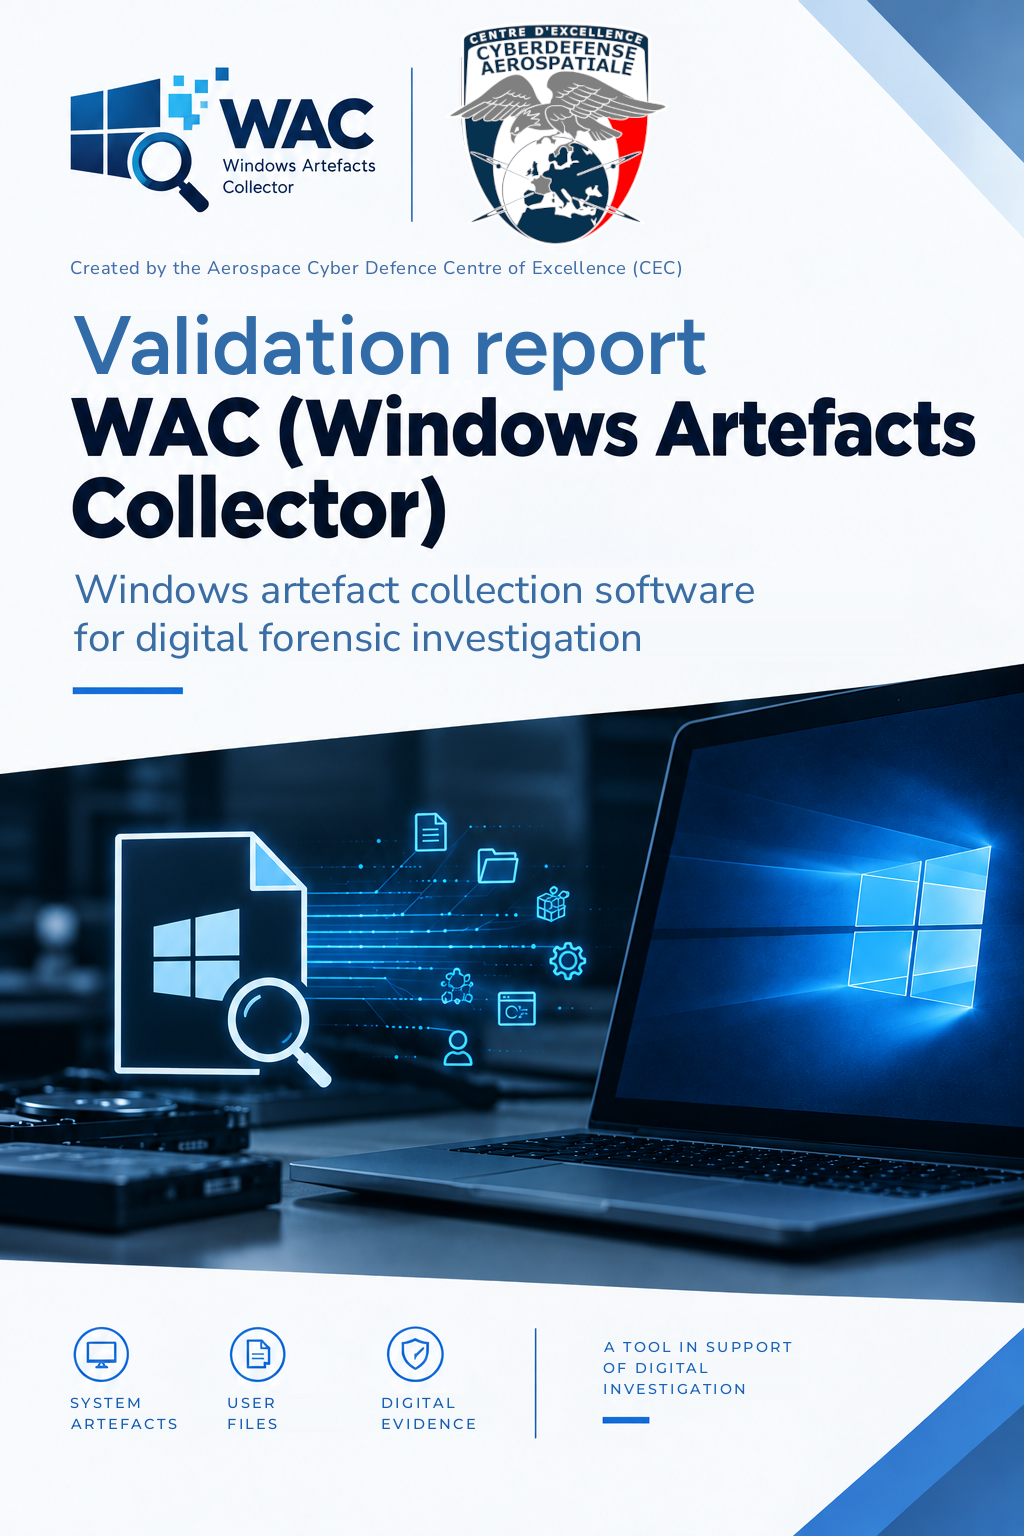
\includegraphics[width=\paperwidth]{cover_validation_EN.png}};
\end{tikzpicture}
\end{titlepage}

% ============================================================ INFORMATION PAGE
\thispagestyle{empty}
\vspace*{\fill}
{\color{marine}\Large\bfseries WAC — Windows Artefacts Collector}\par
{\color{bleu}Validation report}\par
\medskip
\begin{tabular}{@{}ll@{}}
Software version & 1.3.1 \\
Document edition & September 2026 \\
Publisher & Aerospace Cyber Defence Centre of Excellence (CEC) \\
          & French Air and Space Force Academy, Air Base 701, Salon-de-Provence \\
\end{tabular}

\bigskip
{\small\color{gris}This document lists the checks that establish the quality
of \wac{}: those \wac{} runs itself during every collection, the test programs
that confront its decoders with a reference, and the automatic checks of its
outputs. For each, it states what is compared, against what, the reference
result and the defects it has already caught. It also states what these checks
do not guarantee. How to run each test is described in the \emph{Testing
guide}.}
\vspace*{2cm}
\clearpage

\pagenumbering{arabic}
\tableofcontents

% ============================================================ 1
\chapter{The approach}

\section{Why valid JSON proves nothing}

\wac{} produces JSON files meant for a forensic report. Their validity says
almost nothing about their accuracy: a field read at the wrong offset, a date
interpreted in the wrong time zone, a name decoded in the wrong code page, a
wrong decompression all give perfectly valid JSON, and wrong. The most serious
defects found in \wac{} were all of that kind. None showed at run time; each
only appeared when a value was confronted with an \textbf{independent source}.

\wac{}'s validation therefore rests on one principle: every piece of data that
can be cross-checked is, by a means that shares nothing with the code under
test.

\section{Four levels of checks}

\begin{description}[leftmargin=0pt,itemsep=0.5em]
  \item[The checks built into \wac{}] (chapter~\ref{ch:integres}): run during
    every collection, on the examined machine. They refuse inconsistent data
    rather than publish it, and attest the integrity of the exhibits taken.
  \item[The test programs] (chapter~\ref{ch:harnais}): sixteen executables
    that confront each decoder with a reference — the Microsoft function it
    replaces, a published standard or another implementation — or that prove
    a parser never reads outside its buffer.
  \item[The automatic cycle and its checks] (chapter~\ref{ch:cycle}): a full
    collection in a Windows~11 virtual machine, then \fichier{check-json.py},
    which checks the validity of the outputs and confronts them with one
    another and with external sources.
  \item[Cross-checks on a real collection] (chapter~\ref{ch:reel}): what a
    fresh virtual machine does not contain (old logs, fragmented files, exotic
    names) is checked on the data of a real machine, processed locally.
\end{description}

\section{The development rules that go with them}

\begin{enumerate}
  \item \textbf{A fix comes with the test that would have caught the defect},
    and that test is checked both ways: it passes on the fixed code, and it
    fails when the defect is reintroduced. A test never seen failing proves
    nothing.
  \item \textbf{The build is warning-free}, with \texttt{-Wall -Wextra}
    enabled. The warnings also served as a to-do list: each one marked a field
    decoded then dropped.
  \item \textbf{After any change, the new collection is compared with the
    previous one}, artefact by artefact: an artefact gone from 1,522 entries to
    573 lights no warning, only the comparison shows it.
  \item \textbf{Every input is hostile}, including a file of the examined disk:
    every read is bounded by the real size of the buffer, never by a length
    announced in the data.
  \item \textbf{A field without a value is not emitted}: an empty or null key
    would read as data found, or as a failed read.
\end{enumerate}

% ============================================================ 2
\chapter{The checks built into WAC}\label{ch:integres}

These checks are part of the collection program. They run during every
collection, and their result is recorded in \fichier{investigation.json},
operation by operation, with its return code and the trace it leaves on the
examined system.

\section{Before any extraction}

\begin{itemize}
  \item Windows version (10 or later) and effective administrator rights
    (elevated token);
  \item usable collection location and free space, checked \emph{before} the
    first extraction: a collection stopped for lack of space would leave an
    incomplete exhibit store.
\end{itemize}

\section{Raw reading of the NTFS volume}

Locked files (hives, logs) are read directly from the volume, bypassing the
Windows file system. Every structure read is checked before use:

\begin{itemize}
  \item \texttt{FILE} signature of every \fichier{\$MFT} record and
    \texttt{INDX} signature of every index block, then check of the
    \emph{fixups} (update sequence array): every 512-byte stride must end with
    the record's sequence number. A record \emph{torn} by an interrupted write,
    a mix of two versions, is refused instead of being read as plausible
    data;
  \item LZNT1 and WOF decompression bounded by the expected size of each unit:
    a unit that does not produce the expected number of bytes is an error, not
    data silently truncated;
  \item extracted size compared with the size declared by the \texttt{\$DATA}
    attribute: their difference, published in the manifest, reveals a
    truncated extraction a fingerprint alone would not show;
  \item attributes looked for in the extension records too
    (\texttt{\$ATTRIBUTE\_LIST}): a directory whose \texttt{\$INDEX\_ROOT}
    NTFS had moved, the case of thousands of WinSxS components, was reported
    unreadable (4,569 directories of a Windows~11);
  \item released index blocks skipped, per the index's \texttt{\$BITMAP}:
    they can keep stale entries;
  \item every attribute read bounded by the attribute's real size,
    \texttt{\$STANDARD\_INFORMATION} included;
  \item the source file's dates read in \texttt{\$STANDARD\_INFORMATION}
    \emph{and} in \texttt{\$FILE\_NAME}: a program forging the former
    (\emph{timestomping}) leaves the latter untouched, and the gap shows in the
    manifest.
\end{itemize}

\section{Registry hives}

\wac{} reads the hives with its own reader, linked into the executable, and not
with a library of the examined machine.

\begin{itemize}
  \item base block: \texttt{regf} signature, checksum (exclusive OR of the
    first 127 words), primary and secondary sequence numbers. A hive whose logs
    have not been replayed is \textbf{refused}: read as it is, it would give
    stale keys without any error;
  \item replay of the transaction logs (\texttt{.LOG1}/\texttt{.LOG2}):
    signature and sequence chaining of every entry; an entry out of the chain
    is discarded and counted; an undo journal is written before any change, so
    that the raw copy can be rebuilt;
  \item every offset read in the hive is checked against the file's real
    size, and a subkey pointing to one of its ancestors is refused: a walk
    cannot loop on a forged hive.
\end{itemize}

\section{Exhibit integrity: the exhibit store}

Every extracted exhibit is placed in an \emph{exhibit store} that is never
reopened for writing; all the work is done on a second copy.

\begin{itemize}
  \item three fingerprints per exhibit (MD5, SHA-1, SHA-256), computed while
    reading the volume;
  \item the working copy is checked by its SHA-256 against what was read from
    the volume, not against a re-read of the exhibit store;
  \item the manifest identifying the exhibits is sealed by a second file
    carrying its fingerprint: a retouched manifest is detected;
  \item a failed extraction is recorded too: an exhibit missing from the
    manifest would read as never looked for;
  \item the dates of a file artefact (Prefetch, shortcut, jump list) are the
    source file's, recorded in the manifest, never those of the working copy,
    which are the collection's;
  \item a separate conversion (\opt{convert}) checks the seal and every
    exhibit's SHA-256 \emph{before} any read, refuses the store at the first
    difference, and only accepts exhibit paths that stay inside the store.
\end{itemize}

A third party can check the exhibit store without \wac{}, with the scripts
\fichier{verify-exhibits.ps1} (English messages) and
\fichier{verifier-consigne.ps1} (French messages), shipped with the user
documentation: they check the seal, then the fingerprint of every exhibit; an
authenticated binary read but not copied (``fingerprint only'') is counted
apart, having no file.

\section{Authenticity of binaries}

With the \opt{binary} option, \wac{} takes the binaries cited by the
artefacts, except those it establishes as signed by Microsoft. That decision
rests on a complete verification, done by \wac{} itself: RSA signature of each
security catalog, certificate chain up to a Microsoft root, Authenticode
digest of the file found in a verified catalog, or embedded signature. The
catalogs read are those of \path|CatRoot|, of the components
(\path|WinSxS\Catalogs|) and of the servicing packages; the signers accepted,
those Microsoft uses for its own code, \texttt{.NET} included. The files of a
Store application are verified through their package's signature and block
map, 64~KiB block by block. A file whose authenticity is not established is
collected: doubt leads to collecting, never to discarding. The catalogs,
signatures and maps that justified not collecting a file go into the store;
every PE carries its build in the manifest (\texttt{TimeDateStamp},
\texttt{SizeOfImage}), the key of Microsoft's symbol server from which its
identical content can be fetched again. With \opt{binary-all}, everything is
collected, and the verdict is recorded for each executable.

\section{Event logs}

Signature of the file, of each chunk and of each record. Every physical chunk
of the file is walked, not only those the header declares: a log not properly
closed thus yields the records it does not count. An unreadable chunk is
reported and skipped; it no longer stops the reading of the file.

\section{Decoding the artefacts}

\begin{itemize}
  \item every read is bounded by the size of the buffer; an unreasonable
    number of elements in a list of values (beyond 65,536) is refused rather
    than walked;
  \item an impossible date (month~13, hour~25) or one outside the
    \texttt{FILETIME} range gives an absent date, hence not emitted, and never
    an arbitrary value;
  \item every local date carries the offset in force \emph{at its date},
    according to the daylight saving rules of the examined machine, year by
    year;
  \item the SIDs are named from the evidence alone (SAM, well-known SIDs,
    service SIDs, profiles), never by asking the system or the network:
    \texttt{LookupAccountSidW} queried the domain controller for a SID the
    machine did not know, a trace of the collection on another machine. The
    build fails if \fichier{WAC.exe} imports a name-resolution function;
  \item a GUID the reference table does not know is named from the examined
    machine's hives (machine classes, known folders, each user's classes);
    unknown everywhere, it is published without a name, never with a
    placeholder text.
\end{itemize}

% ============================================================ 3
\chapter{The test programs}\label{ch:harnais}

Sixteen executables, left out of \wac{}'s build by their
\fichier{\_test.cpp} suffix and built by \texttt{build-windows.sh --test}.
Each targets one component and confronts it with a judge that shares nothing
with it.

\section{Format harnesses}

\begin{longtable}{@{}L{4.6cm}L{3.8cm}L{6.6cm}@{}}
\toprule
\textbf{Program} & \textbf{Judge} & \textbf{Reference result} \\
\midrule
\endhead
\texttt{sha\_test} & FIPS~180-4 vectors, independent implementation &
  SHA-1 and SHA-256 conform, including lengths 55 to 128 bytes, which exercise
  the padding \\
\texttt{lznt1\_test} & Microsoft's compressor (\texttt{RtlCompressBuffer}) &
  16 compressed units out of 16 conform, 1,048,576 bytes identical \\
\texttt{lzx\_test} & Microsoft's compressor (\texttt{compact /exe:lzx}) &
  646 chunks out of 646 matching (three files); 235,707 truncated or damaged
  inputs without an out-of-bounds read (sanitizers) \\
\texttt{xpress\_test} & Microsoft's compressor &
  137 compressed chunks out of 137 conform, byte for byte \\
\texttt{wevt\_test} & files of a real event provider &
  the whole message production chain checked, substitution marks included \\
\texttt{event\_messages\_test} & SOFTWARE hive and binaries of the machine &
  the same chain, step by step, starting from the hive \\
\texttt{evtx\_test} & \texttt{python-evtx}, independent implementation &
  record by record; whole chain identical when streamed and in memory (26~MB
  peak against 1,281~MB) \\
\texttt{offline\_registry\_test} & Microsoft's \fichier{offreg.dll} &
  18 hives, ten of them from a real machine: 1,273,652 keys and 2,456,139
  values identical \\
\texttt{system\_conversions\_test} & the Windows functions replaced &
  9,861,570 comparisons, no difference (details below) \\
\texttt{consigne\_test} & the exhibit store itself, before and after &
  exhibit store byte-identical after the working copy was modified; seal
  conforms; exhibit paths confined to the store \\
\texttt{ntfs\_fixup\_test} & hand-built records, independent check &
  sound records restored to the byte, torn records and malformed arrays
  refused, 20,000 random records against a forbidden page: 44,610 checks, no
  failure \\
\texttt{json\_test} & WAC's JSON writer & identical round trip, 26 files of a
  collection read back and rewritten to the byte, malformed texts refused,
  200,000 mutations without an out-of-bounds read (sanitizers) \\
\texttt{raw\_hive\_test} & Windows's \texttt{reg load} &
  the extracted hive is refused before repair and accepted after: the test
  fails both ways if it must \\
\texttt{authenticode\_test} & \texttt{Get-Authenticode}\allowbreak\texttt{Signature} &
  2,233 binaries: 2,126 authenticated by both, 99 collected by both, no file
  accepted by \wac{} and rejected by Windows; 462 PowerShell and 11 WSH
  scripts conform \\
\bottomrule
\end{longtable}

\section{Conversions: \texttt{system\_conversions\_test} in detail}

\wac{} depends on five system libraries only (\fichier{ADVAPI32},
\fichier{KERNEL32}, \fichier{msvcrt}, \fichier{Secur32}, \fichier{WTSAPI32}),
needed to query the running system. The conversions it used to ask of other
libraries of the examined machine are done by its own code, and this program
confronts them with the Windows functions they replace:

\begin{itemize}
  \item service SIDs, computed offline, compared with
    \texttt{LookupAccountNameW} for the 273 services of the machine;
  \item GUIDs, SIDs both ways, OLE dates, property names (a table of 1,698
    entries generated from the Windows schema);
  \item FAT dates, on every possible date;
  \item daylight saving time: offset both ways on the \textbf{141 time zones}
    of Windows, with their rules year by year, at every transition from 1980 to
    2035 (hour skipped, hour repeated, change of rule on 1~January);
  \item reading of the \fichier{TimeZoneInformation} key, compared with
    \texttt{GetTimeZoneInformation};
  \item time zone rules forged at random: no overflow.
\end{itemize}

Intended, documented differences: \wac{} refuses a SID text Windows would
truncate, and a non-numeric OLE date for which Windows returns a meaningless
time.

\section{Robustness harnesses}

A parser reads at offsets the file itself declares. On a truncated or forged
file, a read outside the buffer does not crash on its own: it reads the
neighbouring memory and publishes it, in valid JSON. The robustness harnesses
make it crash: each input is placed against a forbidden memory page, once at
its end, once at its start. A single byte read outside the input stops the
test. A watchdog also stops a parser that does not end.

Each file is parsed whole, in its truncations, and in randomly corrupted copies
(fixed seed: a failure reproduces identically).

\begin{longtable}{@{}L{4.2cm}L{6.4cm}L{4.4cm}@{}}
\toprule
\textbf{Program} & \textbf{Files of a real machine} & \textbf{Inputs parsed} \\
\midrule
\endhead
\texttt{lnk\_test} & 220 shortcuts & 546,214 \\
\texttt{parsers\_test} & 48 automatic jump lists & 175,585 \\
 & 23 custom jump lists & 79,036 \\
 & 307 Prefetch files & 1,246,491 \\
 & 4 registry hives & 16,207 \\
\bottomrule
\end{longtable}

Result: no read outside the buffer, no endless loop.

% ============================================================ 4
\chapter{The automatic cycle and its checks}\label{ch:cycle}

\section{The cycle}

\fichier{vmtest/run-wac-test.sh} runs, with no interaction at all, a full
collection in a Windows~11 virtual machine (real NTFS, real registry):

\begin{enumerate}
  \item with \opt{build}, warning-free build of \wac{} and of the test
    programs;
  \item validation of the raw extraction of a hive: \texttt{reg load} must
    refuse it before repair and accept it after;
  \item run of \wac{} with SYSTEM rights; the exit code is checked, and the
    trace is searched for any unhandled exception;
  \item retrieval of the outputs, of the collection log and of the list of
    files actually present in the exhibit store;
  \item run of \fichier{check-json.py};
  \item collection only (\opt{collect} \opt{events} \opt{binary}, or
    \opt{binary-all}), which must convert nothing; check of the store by
    \fichier{verify-exhibits.ps1}; conversion of a store with one retouched
    exhibit, which must be refused before any read; conversion, checked by
    \fichier{check-json.py}; second conversion, whose JSON files must be
    identical to the first's, byte for byte.
\end{enumerate}

\section{The checks of \texttt{check-json.py}}

The script first checks the JSON validity of every file and the form of the
Windows paths (a double escaping shows after parsing). It then confronts values
computed by \wac{} with independent values: another piece of data of the same
collection, or an external source. Each check below was written after a real
defect, which it caught.

\begin{longtable}{@{}L{6.6cm}L{8.4cm}@{}}
\toprule
\textbf{Check} & \textbf{Defect it caught} \\
\midrule
\endhead
\multicolumn{2}{@{}l}{\textit{Dates}} \\
\texttt{X} / \texttt{XUtc} pairs, lists included, naming the same instant
  & double time-zone shift (sessions, shortcuts, installation date); Prefetch
  run times labelled \texttt{+02:00} instead of UTC (1,273 values 2~h off) \\
offset of every local date / IANA time zone database
  & every date labelled with the collection day's offset (106 winter dates at
  \texttt{+02:00}); daylight saving dates of the SYSTEM hive read in the wrong
  layout \\
no session earlier than the system boot & a two-hour shift on the sessions;
  later, a boot time 3.5~s late \\
boot time / Kernel-General~12 event & two independent sources of the same
  instant: 0.00~s apart \\
ShimCache date / NTFS date of the file in the manifest & a UTC date treated as
  local \\
no event later than the collection & shift or misreading of an event date \\
FAT dates without a fraction and with even seconds; Amcache text dates
  without a fraction & every date written with seven digits of fraction,
  claiming a precision the source does not have (808 dates) \\
dates of BAM, UserAssist, USBSTOR and Amcache / \texttt{taskkill} run by
  the harness, Prefetch, \texttt{Get-PnpDeviceProperty}, PE headers & these
  four artefacts store UTC, read as local time: all their dates 2~h off; BAM
  and UserAssist emptied by a regression of the value reading \\
\multicolumn{2}{@{}l}{\textit{Decoding}} \\
output key names in English, without abbreviation & \texttt{NbVolumes},
  \texttt{DateLocale}, \texttt{executionTime}: an abbreviation, a French word,
  a lower-case initial \\
identifier and serial number of a USB key / \texttt{Get-PnpDevice} & no key
  carried its serial number, vendor or product: they are in the key names, not
  in values \\
Prefetch hash / suffix of its file name & 65 wrong hashes out of 270
  (hexadecimal without padding) \\
Prefetch \texttt{\textbackslash VOLUME\{guid\}} paths resolved & 20,066 paths
  out of 20,066 unresolved \\
DestList entries / jump list shortcuts & the first 15 entries of every list
  lost (573 shortcuts published out of 1,522) \\
machine name of the events / \fichier{OperatingSystem.json} & check of the
  BinXML decoding, on two unrelated sources \\
record identifiers unique per log & a stale chunk read again \\
unresolved \texttt{\%\%nnnn} references in messages & a provider's parameter
  file not loaded (3,780 messages) \\
RID found at the end of the rebuilt SID & reading of the SAM database \\
service states and types, presence of drivers & enumeration filters mistaken
  for states \\
no process carries \fichier{WAC.exe} among its modules & the tool's modules
  attributed to the Idle process \\
plausible \fichier{\$MFT} references & decoding of the shortcuts' extension
  blocks \\
mounts / Windows' reading of the key (\texttt{reg query}) and partitions
  (\texttt{Get-Partition}) & 6 mounts out of 7 published as ``\textbackslash{}''
  (device paths decoded as ANSI) \\
SID names / \texttt{Get-LocalUser}, \texttt{Get-LocalGroup} & names asked
  of the running system, even of the domain controller, and translated into
  the workstation's language (``Système'') \\
GUIDs unknown to the table / three GUIDs registered by the harness, one per
  source & ``Unmapped GUID'' published as a name, among them 18 COM handlers of
  the VM's tasks, named in its hive \\
\multicolumn{2}{@{}l}{\textit{Exhibit store and replay}} \\
seal / real fingerprint of the manifest & a retouched manifest \\
three fingerprints per exhibit, consistent counts & an unidentified exhibit \\
files present in the exhibit store / manifest & 209 exhibits added after
  sealing, which every other check let through \\
no hive both replayed and repaired & a replay that does not align the
  sequences \\
an undo journal for every replay & a raw copy impossible to rebuild \\
\multicolumn{2}{@{}l}{\textit{Raw reading, separate collection and conversion}} \\
SHA-256 of files read raw / \texttt{Get-FileHash} & safeguard of the reading by
  batches of contiguous clusters \\
Prefetch dates / dates given by Windows & 0 out of 335 matching: dates of the
  working copy, the minute of the collection \\
executables of System32 and SysWOW64 / manifest of a \opt{collect} \opt{binary}
  & 6,446 missing out of 8,540 (\texttt{\$INDEX\_ROOT} in an extension
  record, names of hard links not declared) \\
catalogs cited in a verdict / exhibits of the store & 170 out of 170 missing
  (label ``catalog'' looked for as ``catalogue'') \\
\wac{}'s Microsoft verdicts / \texttt{Get-AuthenticodeSignature} & safeguard: a
  wrong verdict would leave a binary out of the store \\
copy of a Store package: untouched, modified, added file & verification through
  the signed block map \\
dates of a script forged back to 2001 / \texttt{\$STANDARD\_INFORMATION} and
  \texttt{\$FILE\_NAME} & safeguard: a forgery must stay visible \\
retrieval keys / PE headers read by PowerShell & safeguard of the retrievable
  content \\
\opt{binary-all}: copy and verdict of every executable & package check too
  strict under \opt{binary-all} \\
retouched exhibit / refusal of the conversion & safeguard of the check before
  reading \\
two conversions of one collection & dates read on the working copy, rebuilt at
  each conversion \\
\bottomrule
\end{longtable}

\section{Reference result}

Last cycle, 25 September 2026, on version 1.3.1 (Windows~11, Paris time zone),
no failure and no warning:

\begin{itemize}
  \item \textbf{full run} (\opt{events} \opt{binary}, 4~min~33~s): 24 valid JSON
    files out of 24 produced, USBSTOR included (the harness attaches a virtual
    USB key on every cycle, so that a recreated test machine knows one too);
    62 checks passed, among them 4,090 local dates confronted with the IANA
    database and 170,344 events decoded from 404 logs; 1,640 exhibits, exactly
    those of the manifest, seal conforms;
  \item \textbf{collection only} (\opt{collect} \opt{events} \opt{binary},
    16~min~39~s): nothing converted; 43,513 executables read, 27,958 authenticated
    and not copied, 12,700 Windows differential files, 2,508 collected
    (676~MB); 6,461 exhibits verified by \fichier{verify-exhibits.ps1}; a
    retouched exhibit refused before any read;
  \item \textbf{conversion} (\opt{convert}, 43~s): 75 checks passed, among
    them the 8,539 executables of System32 and SysWOW64 present in the
    manifest, 637 retrieval keys equal to the PE headers, a timestomped script
    visible (\texttt{\$STANDARD\_\allowbreak INFORMATION} of 2001, \texttt{\$FILE\_NAME} of the day), the Store
    package verification; a second conversion gives identical JSON files, byte
    for byte;
  \item \textbf{\opt{binary-all}} (previous cycle): 58,509 executables copied,
    each with its signature verdict.
\end{itemize}

% ============================================================ 5
\chapter{Cross-checks on a real collection}\label{ch:reel}

A fresh virtual machine produces neither fragmentation, nor old jump lists,
nor exotic file names, nor damaged logs. Several defects only showed on a real
machine, confronted with an independent source:

\begin{longtable}{@{}L{5.4cm}L{9.6cm}@{}}
\toprule
\textbf{Cross-check} & \textbf{What it showed} \\
\midrule
\endhead
jump lists / \texttt{olefile} & the streams are named ``1'' to ``f'', not
  ``01'' to ``0f'' \\
shortcut target / DestList entry & a wrong code page and an ignored Unicode
  path \\
logs / \texttt{python-evtx} & a chunk with a wrong signature stopped the
  reading of the whole file (14 records read out of 270) \\
EVTX chunks / their CRC32 & one-off check: the 1,505 chunks of the 404 logs of
  the test machine are intact \\
hives / \fichier{offreg.dll} & 1,273,652 identical keys \\
binaries / \texttt{Get-AuthenticodeSignature} & no undue authentication \\
old output / new one & the same files decoded by the current code, compared
  after normalisation \\
\bottomrule
\end{longtable}

\begin{note}
A real collection contains personal data. It is processed locally; a temporary
copy in the virtual machine or in a working folder is deleted after use, and
nothing of it enters the source repository.
\end{note}

% ============================================================ 6
\chapter{What these checks guarantee}

\section{Guarantees}

\begin{itemize}
  \item \textbf{Exhibit integrity}: every exhibit is identified by three
    fingerprints, the working copy is checked against the reading of the
    volume, the manifest is sealed, and the exhibit store is never modified
    (\texttt{consigne\_test}, checks of the cycle).
  \item \textbf{No writing to the examined system}, apart from the unavoidable
    traces of a collection on a running system, all recorded in
    \fichier{investigation.json} with the expected trace.
  \item \textbf{Accuracy of the decoders}: where a reference exists — hive
    reader, decompressions, fingerprints, conversions, time zones, authenticity
    of binaries — results identical to it on the volumes stated.
  \item \textbf{Robustness}: no shortcut, jump list, Prefetch or hive parser
    reads outside its buffer or loops, on more than two million truncated or
    corrupted inputs.
  \item \textbf{Consistency of the outputs}: every possible cross-check
    between two artefacts, or between an artefact and an external source, is
    run in every cycle.
  \item \textbf{Independence from the examined machine}: \wac{} borrows no
    library from it to interpret the evidence.
\end{itemize}

\section{Limits}

\begin{attention}
These checks do not prove the absence of defects. They prove that the defects
they target are absent, on the data they have seen.
\end{attention}

\begin{itemize}
  \item \textbf{Completeness}: an empty artefact cannot be told apart from a
    machine without traces. Only the comparison between two collections, or
    with a machine whose content is known, measures it.
  \item \textbf{Data the test machine does not hold}: MTP devices,
    files spread over several \fichier{\$MFT} records
    (\texttt{\$ATTRIBUTE\_LIST}), very large volumes. They are to be validated
    on real systems.
  \item \textbf{Artefacts without a reference}: when no independent tool reads
    a format, its accuracy rests on the internal cross-checks and on the public
    documentation of the format.
  \item \textbf{Time zones}: the confrontation with the IANA database covers
    the zones whose rules agree with Windows's over the period checked
    (Western Europe, United States, UTC); the others are checked against
    Windows only.
  \item \textbf{MSVC build}: the Visual Studio project is maintained, but the
    checks are made on the MinGW build, the one delivered.
\end{itemize}

\end{document}
